%*----------- SLIDE -------------------------------------------------------------
\begin{frame}[t]{ROS - Robot Operating System} 
  \centering
  
\includegraphics[width=.9\linewidth]{ros_pr2.jpeg}
  
  \vspace{.5cm}
  O ROS é um conjunto de bibliotecas e ferramentas de software que nos ajudam a desenvolver aplicações robóticas. Possui desde ferramentas de visualização até drivers e algoritmos de Estado-da-Arte, de forma que não precisamos criar tudo do zero.

  E tudo isso é \textbf{Open Source}!
\end{frame}


%*----------- SLIDE -------------------------------------------------------------
\begin{frame}[t]{Distribuições ROS} 
  \centering
  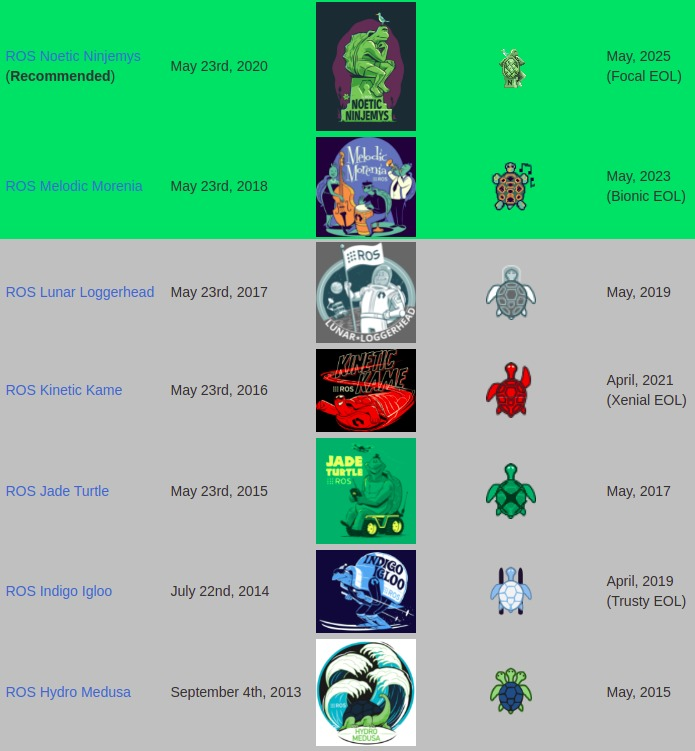
\includegraphics[width=.42\linewidth]{distribuicoes_1.jpeg}
  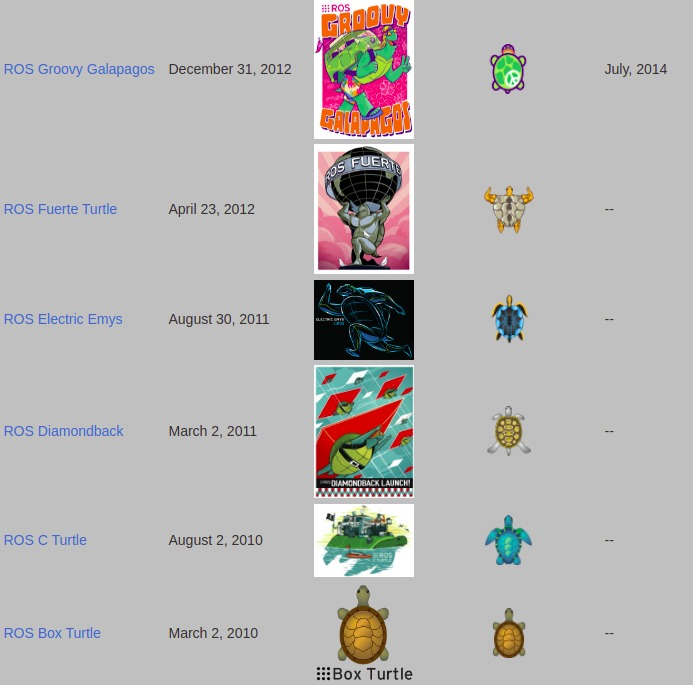
\includegraphics[width=.42\linewidth]{distribuicoes_2.jpeg}
\end{frame}


%*----------- SLIDE -------------------------------------------------------------
\begin{frame}[t]{Robôs que utilizam ROS} 
  \centering
  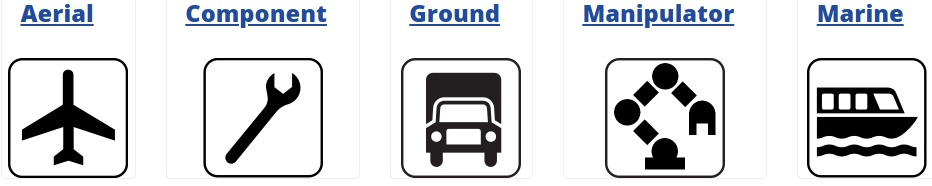
\includegraphics[width=.42\linewidth]{aplicacoes.jpeg}
  
  \href{https://robots.ros.org/}{https://robots.ros.org/}


\end{frame}


%*----------- SLIDE -------------------------------------------------------------
\begin{frame}[t]{Por que utilizar o ROS?} 
  \begin{columns}
    \column{.6\textwidth}
    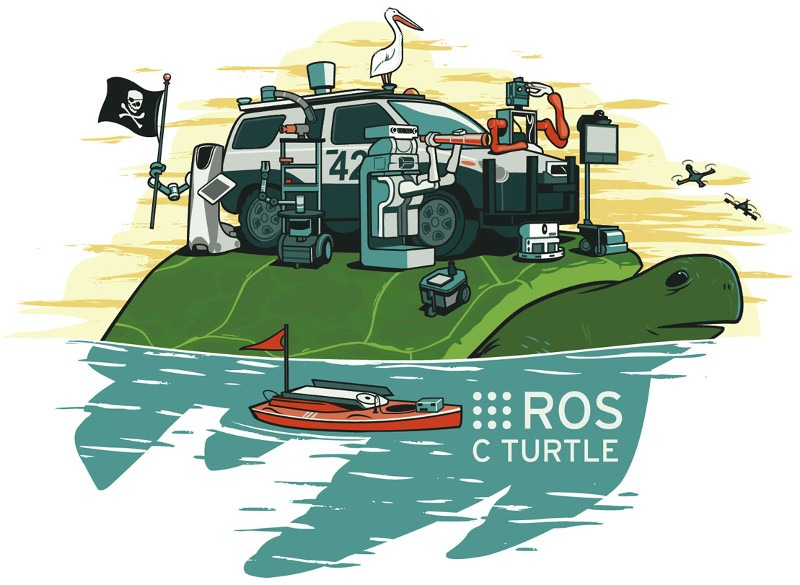
\includegraphics[width=\textwidth]{ros_robots_turtle.jpg}
    
    \column{.4\textwidth}
    \begin{itemize}
      \item ROS é de uso geral, você pode utilizá-lo na aplicação que desejar;
      \item Possui uma gama de ferramentas úteis para simulação e visualização;
      \item Possui pacotes para tudo do que se possa imaginar;
      \item Podemos controlar diversos robôs, fazendo com que eles se comuniquem
    \end{itemize}

  \end{columns}
\end{frame}


%*----------- SLIDE -------------------------------------------------------------
\begin{frame}[t]{Gazebo} 
  \centering
  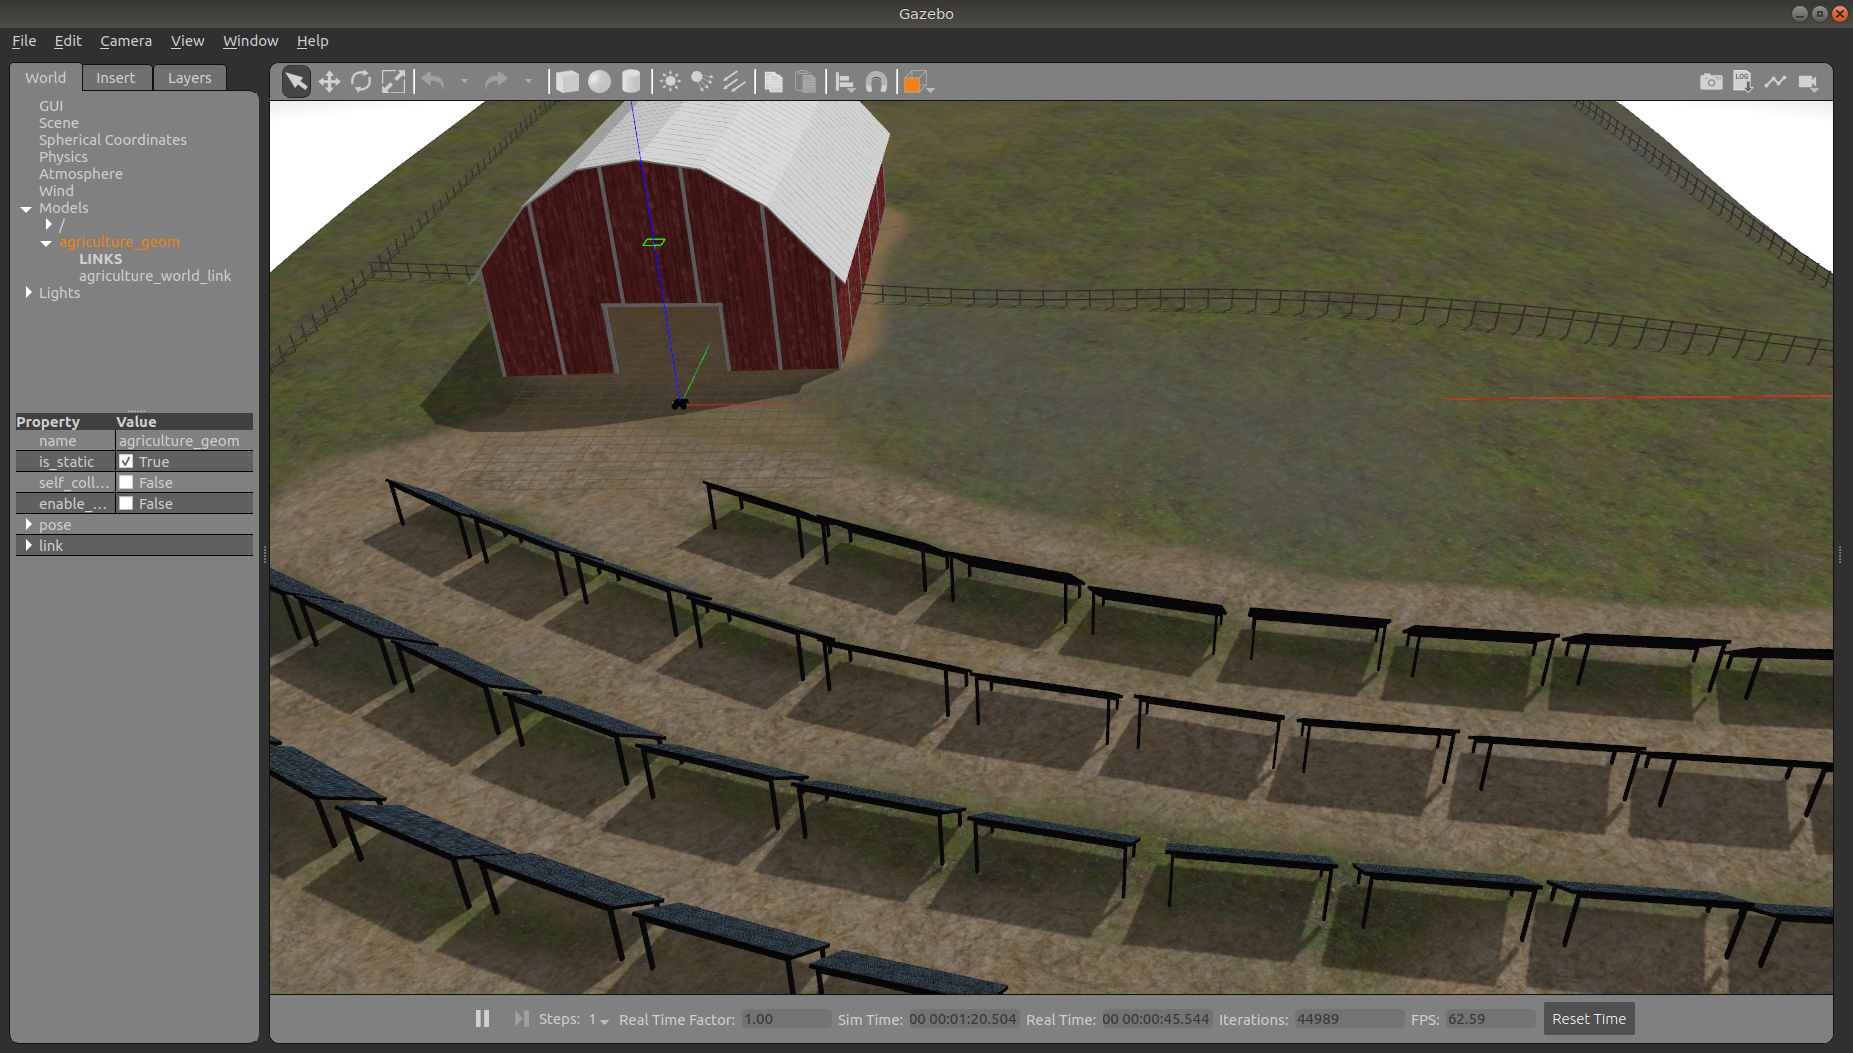
\includegraphics[width=.62\linewidth]{agriculture_world.png}
  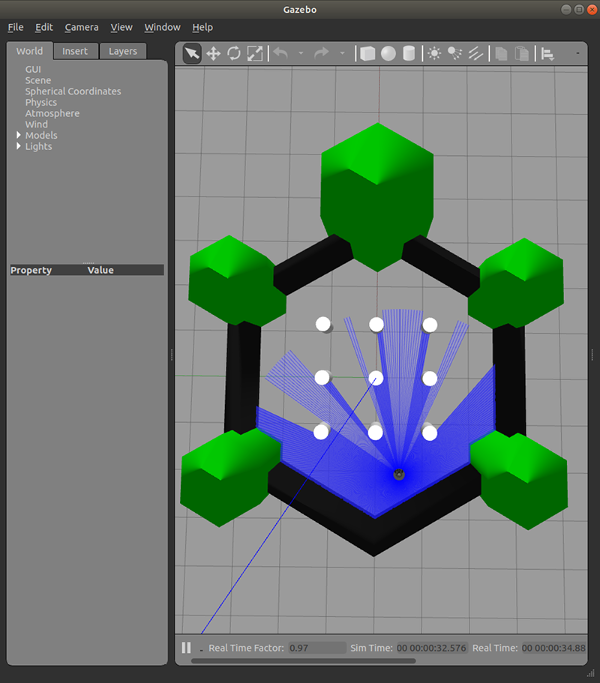
\includegraphics[width=.308\linewidth]{gazebo_world.png}
  
  \begin{columns}
    \column{.06\textwidth}
    
\includegraphics[width=\linewidth]{gazebo_logo.png}

    % \column[0.1cm]{.8\textwidth}
    
    Gazebo é um simulador 3D robusto e de código aberto, muito utilizado para simulação de robôs, tornando possível o teste de seus controles e algoritmos em ambientes próximos do real.
  \end{columns}

\end{frame}


%*----------- SLIDE -------------------------------------------------------------
\begin{frame}[t]{Como funciona o ROS?}

  
\includegraphics[width=.5\textwidth]{ros_logo.png}
  \vspace{.5cm}
  \begin{itemize}
    \item \textbf{Nodes:} Nós são executáveis que utilizam o ROS para se comunicar com outros Nós
    \item \textbf{Messages:} Mensagens são os tipos de estrutura de dados utilizados pelo ROS
    \item \textbf{Topics:} Os nós podem publicar e ler mensagens em Tópicos
    \item \textbf{Master:} Mestre, controla a comunicação entre todos os nós
    \item \textbf{Rosout:} Equivalente do ROS ao stdout
    \item \textbf{Roscore:} Master + rosout + parameter server 
  \end{itemize}

\end{frame}
